\providecommand{\tightlist}{}
\chapter{Proposta}
\section{\textbf{Introdução}}{Introdução}\label{introduuxe7uxe3o}

A classificação automática de metáforas constitui um desafio clássico no
campo do processamento de linguagem natural (PLN), devido à natureza
abstrata e dependente de contexto das expressões metafóricas.
Diferentemente das abordagens tradicionais que buscam identificar a
presença ou ausência de metáforas, este trabalho recebe metáforas já
detectadas em um pipeline prévio e propõe classificá-las em categorias
específicas baseadas no referencial histórico proposto por Fernández
Sebastián (2024). Esta classificação, sustentada teoricamente pelo
estudo qualitativo e erudito das fontes históricas, visa compreender
mais profundamente os padrões e o desenvolvimento das metáforas ao longo
do tempo. Essa tarefa ocorre no contexto da construção de um dataset
diacrônico --- um recurso ainda relativamente raro em PLN --- cuja
curadoria está sendo conduzida por outros membros da equipe. O presente
trabalho contribui com sua expansão e validação por meio da
classificação automatizada das metáforas e da recuperação de evidências
históricas.

Além disso, o projeto contempla dois módulos complementares: o
\emph{Metaphor Classifier}, que classifica e expande o conjunto de
metáforas por meio da recuperação de trechos semanticamente semelhantes
nas fontes históricas; e o \emph{RAG} (Retrieval-Augmented Generation),
responsável por gerar justificativas textuais embasadas, citando
passagens das obras consultadas. Este segundo módulo combina capacidades
avançadas dos modelos grandes de linguagem (LLMs) com mecanismos de
recuperação automatizada de contextos históricos e literários
relevantes. Espera-se, assim, contribuir para uma compreensão mais
fundamentada e transparente de metáforas em corpora históricos,
oferecendo suporte empírico para hipóteses historiográficas. O RAG cumpre 
a função central do trabalho de prova historiográfico, atuando em sua 
função referencial \cite{lewis2020rag}.

\section{\textbf{Objetivos}}{Objetivos}\label{objetivos}

\subsection{\texorpdfstring{\textbf{Objetivo
Geral}}{Objetivo Geral}}\label{objetivo-geral}

Desenvolver e integrar dois módulos: o \emph{Metaphor Classifier},
responsável por atribuir categorias históricas a metáforas previamente
detectadas e expandir o conjunto de exemplos por meio de recuperação
semântica de ocorrências análogas; e o \emph{RAG}, voltado à geração de
justificativas textuais embasadas, citando e recuperando evidências 
históricas relevantes para cada classificação.

\subsection{\texorpdfstring{\textbf{Objetivos
Específicos}}{Objetivos Específicos}}\label{objetivos-especuxedficos}

\begin{enumerate}
\def\labelenumi{\arabic{enumi}.}
\item
  \textbf{Construção de regras de categorização}\\
  Desenvolver regras interpretáveis com base em um documento de
  categorias e exemplos elaborado por historiadores, de modo a
  possibilitar a atribuição automática ou semi-automática de categorias
  históricas a metáforas detectadas.
\item
  \textbf{Metaphor Classifier --- Recuperação de evidências
  históricas}\\
  Dado um conjunto de metáforas detectadas, atribua categorias
  históricas e recupere metáforas similares em contextos históricos,
  compondo pares metáfora~$\leftrightarrow$~evidência textual.
\item
  \textbf{RAG --- Geração de justificativas explicativas}\\
  Desenvolver um segundo módulo capaz de gerar respostas textuais
  explicativas para cada metáfora classificada, citando a evidência
  textual recuperada e a justificando com base na categoria histórica
  atribuída.
\item
  \textbf{Avaliação funcional do pipeline}\\
  Avaliando-os com métricas formais (como F1-score ou precisão, se
  aplicável) ou, se simbólicos, com checklist qualitativo.
\item
  \textbf{Documentação e replicabilidade prática}\\
  Manter documentação clara e progressiva no repositório do projeto,
  incluindo instruções de uso, descrição das etapas e exemplos de
  entrada e saída para cada módulo.
\item
  \textbf{Flexibilidade de escopo e adaptação contínua}\\
  Conduzir o desenvolvimento sob abordagem iterativa e adaptativa,
  permitindo ajustes de rota conforme os dados e insumos forem
  disponibilizados por terceiros, respeitando os marcos definidos no
  cronograma.
\end{enumerate}

\subsection{Escopo do Trabalho}\label{escopo-do-trabalho}

\subsubsection{1 · Entradas externas
(pré-requisitos)}\label{entradas-externas-pruxe9-requisitos}

\begin{table}[htbp]
  \small
  \caption{Entradas externas (pré-requisitos)}    % Tabela 1
  \label{tab:entradas}
  \centering
  \begin{tabularx}{\linewidth}{@{}>{\RaggedRight\arraybackslash}p{2.5cm}
                                    >{\RaggedRight\arraybackslash}X
                                    >{\centering\arraybackslash}p{2.2cm}
                                    >{\RaggedRight\arraybackslash}p{2.4cm}
                                    >{\RaggedRight\arraybackslash}p{3.3cm}@{}}
    \toprule
    Origem & Entregável & Data prevista & Formato & Observação \\ \midrule
    Eduardo   & Embeddings vetoriais das obras históricas & 31 jul 2025 & Parquet / FAISS / Chroma & Recuperação semântica \\[2pt]
    Franciele & Documento de categorias (3 exemplos cada) & 15 ago 2025 & Markdown & Base p/ regras de categorização \\
    \bottomrule
  \end{tabularx}
  \fonte{Elaboração própria.}
\end{table}

\subsubsection{2 · Contribuições diretas do
autor}\label{contribuiuxe7uxf5es-diretas-do-autor}

\begin{table}[htbp]
  \small
  \caption{Contribuições diretas do autor}        % Tabela 2
  \label{tab:contribuicoes}
  \centering
  \begin{tabularx}{\linewidth}{@{}>{\RaggedRight\arraybackslash}p{3cm}
                                    >{\RaggedRight\arraybackslash}X
                                    >{\RaggedRight\arraybackslash}p{4.2cm}@{}}
    \toprule
    Módulo & Descrição resumida & Critério de aceite \\ \midrule
    \textbf{Metaphor Classifier} & Classifica metáforas detectadas e recupera expressões análogas em obras históricas. & $\geq$ 100 pares \textit{(metáfora, evidência, categoria)} gerados; execução end-to-end comprovada \\[2pt]
    \textbf{QuantEval} & Avalia a qualidade e coerência dos pares por checklist ou métricas formais. & Relatório técnico em Markdown com amostra comentada ou validação formal \\[2pt]
    \textbf{RAG} & Gera justificativas textuais baseadas na evidência recuperada. & Executável em $\geq$ 10 metáforas distintas com justificativas coerentes e citação da fonte \\
    \textbf{Docs} & Documentação viva (README, exemplos, instruções) atualizada a cada entrega. & Cada etapa entregue contém documentação correspondente no repositório \\ \bottomrule
  \end{tabularx}
  \fonte{Elaboração própria.}
\end{table}


\subsubsection{3 · Fora do escopo}\label{fora-do-escopo}

\begin{itemize}
\tightlist
\item
  Detecção inicial de metáforas (Classificação Binária)
\item
  Dataset-A (pré-existente)\\
\item
  OCR, interface web\\
\item
  LLM fine-tuned usada no RAG (fornecida por terceiros)
\end{itemize}

\subsubsection{4 · Premissas \&
restrições}\label{premissas-restriuxe7uxf5es}

\begin{itemize}
\tightlist
\item
  VLab-UFSC disponível com GPU/CPU até \textbf{julho/2026}.\\
\item
  Textos históricos em domínio público; nenhuma licença adicional é
  necessária.\\
\item
  Volume de dados modesto (\textless{} 10 GB); notebook pessoal e Google
  Drive são suficientes como redundância.\\
\item
  Se embeddings ou categorias atrasarem, o escopo será reduzido ou o
  autor assumirá tarefas extras.
\end{itemize}

\subsubsection{5 · Cronograma técnico
resumido}\label{cronograma-tuxe9cnico-resumido}

\begin{itemize}
\tightlist
\item
  \textbf{mar--abr 2025}

  \begin{itemize}
  \tightlist
  \item
    Leitura de fundamentos sobre RAG
  \item
    PoC inicial com prompt fixo
  \item
    Leitura dos capítulos 4--7 de Fernández Sebastián
  \item
    Estudo do estado da arte sobre PLN e metáforas
  \item
    Base estruturada inicial do \emph{Metaphor Classifier}
  \end{itemize}
\item
  \textbf{jul--ago 2025}

  \begin{itemize}
  \tightlist
  \item
    Recebimento dos embeddings (Eduardo)
  \item
    Recebimento do documento de categorias (Franciele)
  \item
    Implementação do \emph{Metaphor Classifier}
  \end{itemize}
\item
  \textbf{set--out 2025}

  \begin{itemize}
  \tightlist
  \item
    Expansão do Dataset-B com recuperação de metáforas similares
  \item
    Ajuste das regras de categorização com base nas novas evidências
  \item
    Avaliação funcional do \emph{Metaphor Classifier} (QuantEval)
  \item
    Desenvolvimento do módulo \emph{RAG} (geração de justificativas
    textuais)
  \item
    Redação do Projeto II
  \end{itemize}
\item
  \textbf{dez 2025 -- fev 2026}

  \begin{itemize}
  \tightlist
  \item
    Curadoria de logs e análise de falhas
  \item
    Organização de outputs e documentação técnica
  \item
    Planejamento da redação final do TCC
  \end{itemize}
\item
  \textbf{mar--jun 2026}

  \begin{itemize}
  \tightlist
  \item
    Versão revisada(foco em precisão) dos Scripts
  \item
    Redação da versão completa do TCC final
  \end{itemize}
\item
  \textbf{jun 2026}

  \begin{itemize}
  \tightlist
  \item
    Margem para retorno da banca antes da defesa
  \item
    Preparação da defesa pública (slides, ensaios)
  \end{itemize}
\item
  \textbf{jul 2026}

  \begin{itemize}
  \tightlist
  \item
    Ajustes finais e formatação ABNT
  \item
    Depósito do TCC na BU/UFSC
  \end{itemize}
\end{itemize}

\section{\textbf{Método de Pesquisa}}{Método de Pesquisa}\label{muxe9todo-de-pesquisa}

Adotar-se-á uma abordagem mista, combinando métodos quantitativos e
qualitativos. A dimensão \textbf{quantitativa} será utilizada sempre que
o processo de classificação empregar modelos supervisionados, com
aplicação de métricas como \emph{F1-score}, \emph{precision} e
cobertura. Caso o classificador opere de forma simbólica, a avaliação
seguirá uma abordagem qualitativa baseada em checklist, com inspeção
manual da correspondência entre metáfora, categoria atribuída e
evidência textual recuperada.

A dimensão \textbf{qualitativa} estará presente tanto na definição das
categorias quanto na validação da coerência histórico-conceitual dos
pares gerados (\emph{metáfora~$\leftrightarrow$~evidência}). Nessa etapa, as
classificações e justificativas produzidas pelos módulos serão
analisadas à luz do referencial de Fernández Sebastián, com apoio da
equipe de historiadores do projeto.

Trata-se de um estudo descritivo-exploratório, cujo objetivo principal é
mapear e caracterizar padrões metafóricos diacrônicos com base em fontes
textuais históricas. Não se busca inicialmente estabelecer relações de
causalidade, mas sim levantar regularidades e hipóteses interpretativas
que possam ser testadas posteriormente em estudos historiográficos mais
amplos.

A pesquisa é de natureza aplicada, voltada ao desenvolvimento de módulos
computacionais que integrarão um pipeline mais amplo. Dentre esses
módulos, destacam-se o \emph{Metaphor Classifier}, responsável pela
categorização e expansão do conjunto de metáforas, e o \emph{RAG},
voltado à geração textual explicativa com embasamento rastreável.

Serão utilizadas técnicas modernas de PLN, como \emph{Large Language
Models} (LLMs), vetorização semântica e algoritmos de vizinhança (K-NN).
As ferramentas específicas --- como bibliotecas de vetorização, índices
semânticos ou modelos de geração --- serão escolhidas conforme os
requisitos práticos da implementação.

A execução ocorrerá em ambiente computacional misto, utilizando notebook
pessoal e infraestrutura da UFSC, como o
\href{https://jupyter.vlab.ufsc.br/hub}{VLab da UFSC}, bem como o
repositório colaborativo
\href{https://github.com/iaehistoriaUFSC/metaphoriq}{IAeHistoriaUFSC},
no qual o progresso do projeto será mantido de forma incremental e
documentada.

\section{\textbf{Cronograma}}{Cronograma}\label{cronograma}

\begin{quote}
\textbf{Nota:} O cronograma abaixo parte do pressuposto de que certos
insumos técnicos --- como embeddings vetoriais das obras históricas e
etapas de pré-processamento --- estão sendo desenvolvidos paralelamente
por integrantes da equipe técnica (especialmente Maiko Nunes, Giovanna
Ramalho e Eduardo Goulart). O autor assume a integração desses artefatos
nos módulos sob sua responsabilidade, sem duplicar esforços já em curso.
\end{quote}

\begin{figure}[H]
  \centering
  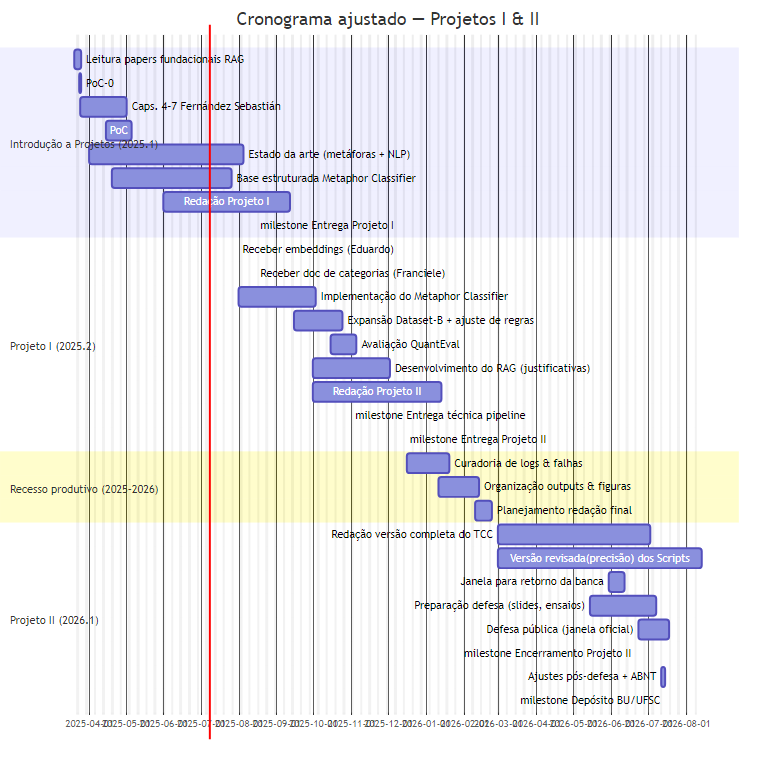
\includegraphics[height=0.7\textheight,keepaspectratio]{pictures/gantt.png}
  \caption{Diagrama de Gantt}
  \label{fig:gantt}
\end{figure}

\section{\textbf{Custos}}{Custos}\label{custos}

Não há custos previstos para a execução deste trabalho, uma vez que
todos os recursos necessários --- incluindo ferramentas de processamento
de linguagem natural, repositórios digitais, infraestrutura
computacional (como o VLab da UFSC) e canais de comunicação --- são
gratuitos, institucionais ou já disponíveis para os membros da equipe.

\section{\textbf{Recursos
Humanos}}{Recursos Humanos}\label{recursos-humanos}

\begin{table}[htbp]
  \small
  \caption{Recursos humanos envolvidos}           % Tabela 3
  \label{tab:rh}
  \centering
  \begin{tabularx}{\linewidth}{@{}>{\RaggedRight\arraybackslash}p{5.5cm}
                                    >{\RaggedRight\arraybackslash}X@{}}
    \toprule
    Nome & Função \\ \midrule
    Rodrigo Bragio Bonaldo & Orientador \\
    Jean Carlo Rossa Hauck & Coorientador/Responsável \\
    Chiru Stefan & Senior Developer \\
    Patricia Biral Varela & Pesquisadora em História \\
    Maiko Ademir Nunes & Desenvolvedor Junior \\
    Giovanna Ramalho & Engenharia de Software \\
    Eduardo Peres Luckner Goulart & Desenvolvedor Junior \\
    Franciele Dias da Silva & Pesquisadora em História com função
    organizacional \\
    Mateus Freitas Borsatti & Pesquisador em História \\
    Letícia Portella Milan & Pesquisadora em História \\
    Éric Gabriel Kundlatsch & Pesquisador em História \\
    Isabella Stersa de Oliveira & Pesquisadora em História \\
    Gilson Mateus Pinto Júnior & Pesquisador em História \\
    Leonardo Nogueira Aucar & Pesquisador em História \\
    Gabriela Graudenz Muller & Linguística \\
    Willian Meurer Welter & Pesquisador em História \\
    Danillo Melo da Fonseca & Pesquisador em História \\
    Alysson Julio Risso da Silva & Pesquisador em História \\
    Marcel Vieira Silva & Pesquisador em História \\
    Thamiris Fátima dos Santos & Desenvolvedor Front-End \\
    Renata da Conceição Aquino da Silva & Pesquisadora em História \\
    Fernanda Lyrio Heinzelmann & Psicologia \\
    Breno Ampáro & Pesquisador em História \\
    Gabriel Choucair Garcia & Pesquisador em História \\ \bottomrule
  \end{tabularx}
  \fonte{Elaboração própria.}
\end{table}

\section{\textbf{Comunicação}}{Comunicação}\label{comunicauxe7uxe3o}

\begin{table}[htbp]
  \small
  \caption{Plano de comunicação}                  % Tabela 4
  \label{tab:comunicacao}
  \centering
  \begin{tabularx}{\linewidth}{@{}>{\RaggedRight\arraybackslash}p{4.8cm}
                                    >{\RaggedRight\arraybackslash}p{1.6cm}
                                    >{\RaggedRight\arraybackslash}p{2.4cm}
                                    >{\RaggedRight\arraybackslash}p{2.8cm}
                                    >{\RaggedRight\arraybackslash}X@{}}
    \toprule
    O que será comunicado & Por quem & Para quem & Meio & Frequência \\ \midrule
    Progresso técnico (pipeline, classificador, RAG) & Autor & Equipe técnica & Reunião Google Meet & Ter 14 h - 16 h semanal \\[2pt]
    Discussões conceituais sobre categorias & Autor & Equipe de História & Reunião Google Meet & Ter 16h30 - 17h30 semanal \\[2pt]
    Dúvidas de código/ferramentas & Autor & Stefan (coorientador técnico) & WhatsApp ou reunião & Sob demanda / semanal \\[2pt]
    Entregas parciais & Autor & Orientador(es) & GitHub / reunião & Ao final de cada etapa \\[2pt]
    Integrações entre módulos & Equipe técnica & Integrador designado & WhatsApp / Discord & Quando necessário \\[2pt]
    Avisos gerais & Autor & Todos & Grupo “IA e História” (WhatsApp) & Assíncrono contínuo \\ \bottomrule
  \end{tabularx}
  \fonte{Elaboração própria.}
\end{table}

\section{\textbf{Riscos}}{Riscos}\label{riscos}

\begin{table}[htbp]
  \small
  \caption{Riscos potenciais do projeto}          % Tabela 5
  \label{tab:riscos}
  \centering
  \begin{tabularx}{\linewidth}{@{}>{\RaggedRight\arraybackslash}p{4.2cm}
                                    >{\centering\arraybackslash}p{1.9cm}
                                    >{\centering\arraybackslash}p{1.5cm}
                                    >{\centering\arraybackslash}p{1.6cm}
                                    >{\RaggedRight\arraybackslash}p{3.1cm}
                                    >{\RaggedRight\arraybackslash}X@{}}
    \toprule
    Risco & Probabilidade & Impacto & Prioridade & Estratégia de resposta & Ações de prevenção \\ \midrule
    Integração complexa entre etapas do pipeline & Baixa & Alta & Média & Modularizar componentes & Revisões técnicas semanais com Stefan \\[2pt]
    Ingestão do dataset diacrônico demanda maior esforço & Alta & Alta & Alta & Reduzir escopo ou redefinir metas & Pilotos incrementais e testes de carga \\ \bottomrule
  \end{tabularx}
  \fonte{Elaboração própria.}
\end{table}
